
\begin{figure}[t]
	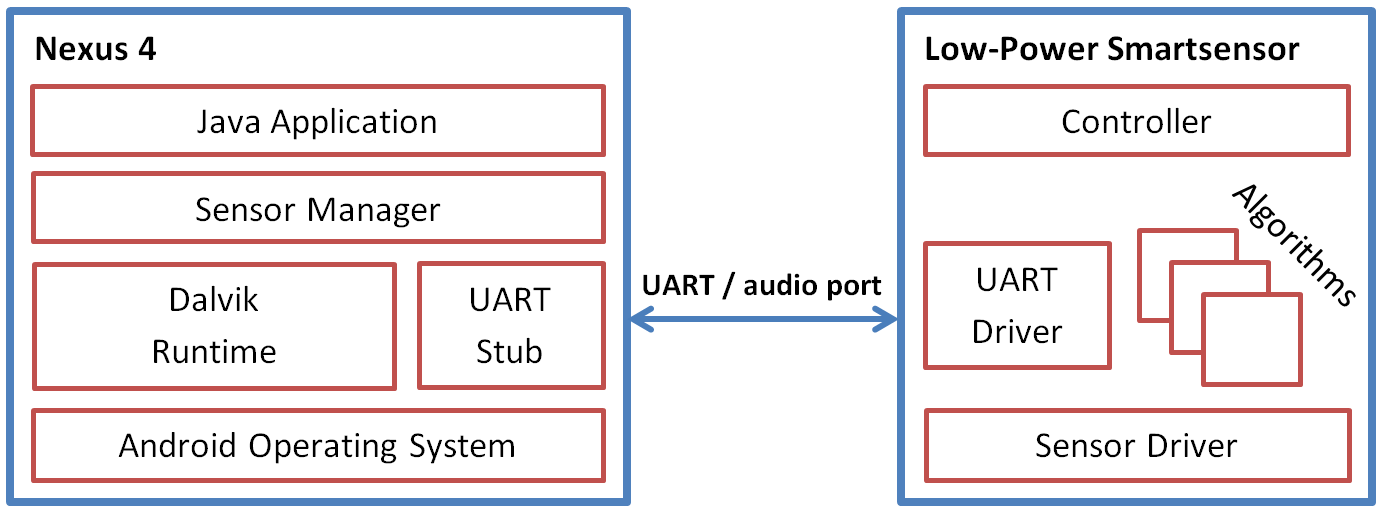
\includegraphics[width=3.1in]{prototype_architecture.png}
	\caption{Prototype architecture.}
    \label{fig:prototypeArchitecture}
\end{figure}

\section{Prototype}
\label{sec:prototype}

We implemented a prototype of our system using a Google Nexus 4 phone
running Android 4.2.2.  The low-power sensor node is implemented using
a Texas Instruments micro-controller board attached to an
accelerometer sensor.  We chose to focus our efforts on the
accelerometer sensor because of its relative simplicity and the
availability of a wide range of accelerometer-based applications on
various mobile application markets.  Figure
\ref{fig:prototypeArchitecture} shows a high-level diagram of the
prototype's architecture.

The Nexus 4 and TI board communicate over the UART port made available
by the Nexus 4 debugging interface via the physical port used by the
audio interface.  The serial connection provides sufficient bandwidth
to support low bit-rate sensors, such as the accelerometer, a
microphone or GPS.  However, extending the prototype to work with
higher bit-rate sensors like the camera would require a higher
bandwidth data bus, such as $I^2C$.

This section describes our extensions to the phone, the
sensor node implementation, and the test
framework we use in our experiments.

\subsection{Nexus 4}
\label{subsec:nexus}

On the Nexus phone we extended Android's SensorManager to include the
new features made available by our system. To prevent a steep learning
curve, our goal was to provide an API very similar to Android's
existing sensors API.  

We extended the Sensor Manager to allow developers to define SCC by building
a pipeline of pre-defined data processing algorithms and configuring their
parameters. The available types of processing algorithms are
described in Subsection~\ref{sec:sensorDataAlgorithms}.

\hl{Silviu: Include API usage example?}

We also created a UART stub to facilitate communication between the
mobile phone and the sensor node. The UART stub is called when
the sensor node detects an event based on its SCC.
In turn, the UART stub is a shell script that notifies the
SensorManager using an Android Intent~\cite{androidintents}.

For our prototype we avoided modifying the Android kernel in any way.
Because the current prototype uses the UART port for communication
with the sensor node, we were able to constrain our implementation to
the user space.  An integrated implementation would likely make use of
a higher bandwidth bus such as the $I^2C$ bus and require a custom
driver.

\bgroup
\def\arraystretch{1.5}
\begin{table*}[t]
\centering
{\small
	\begin{tabular}{| l | c | c |}
		\hline
		\textbf{State}								& \textbf{Average Power Consumption (mW)} 		& \textbf{Average Duration} \\ \hline
		Awake, running sensor-driven application 	& 323 											& N/A \\ \hline
		Asleep 										& 9.7 											& N/A \\ \hline
		Asleep-to-Awake Transition 					& 384 											& 1 second \\ \hline
		Awake-to-Asleep Transition 					& 341 											& 1 second \\ \hline
	\end{tabular}
}
	\caption{Google Nexus 4 power profile.}
	\label{table:powerProfileNexus}
\end{table*}
\egroup

We power profiled the Google Nexus 4.  The results are summarized in
Table~\ref{table:powerProfileNexus}.  During all the measurements, the
device's screen, WiFi and GPS were turned off.  While the device is
sleeping, its power usage is very low, consuming only 9.7 mW.  While
awake, the power consumption is significantly higher, averaging 323
mW.  During our power measurements we noticed that additional energy is
consumed during transitions between the asleep and awake states.  Each
transition takes about 1 second.  During a wake-up transition, the
average power consumption goes up to 384 mW, while during an
awake-to-asleep transition the average power consumption is 341 mW.


\subsection{Sensor Node}
\label{subsec:sensorNode}

The low-power sensor node consists of a driver that talks to
the accelerometer sensor, a set of data processing algorithms, a controller,
and an UART driver for communicating with the phone.  The controller
orchestrates the execution of the algorithms, and uses the UART driver to
wake up the phone when an event is detected by the SCC.  The UART driver
opens a serial port and then uses a TTY to copy the sensor readings
and starts the shell script that notifies the Sensor Manager.


\subsubsection{Sensor Data Processing Algorithms}
\label{sec:sensorDataAlgorithms}

We implemented the following processing algorithms:

\begin{itemize}

	\item {\bf Windowing} Partitioning sensor data into rectangular or Hamming windows.
		
	\item {\bf Transform} Fast Fourier Transform (FFT) from time-domain to frequency-domain.
	  
	\item {\bf Data Filtering} 
		\begin{itemize}
			\item Noise-reduction algorithm based on exponential moving average with 
	  configurable degree of weighting decrease.
			\item FFT-based low-pass filtering.
			\item FFT-based high-pass filtering.
		\end{itemize}

	\item {\bf Feature Extraction} 
		\begin{itemize}
			\item Magnitude of acceleration vector computation.
			\item Zero Crossing Rate computation.
			\item A set of statistical functions, including mean and variance computation.
			\item Determination of magnitude of dominant frequency.
		\end{itemize}

	\item {\bf Admission Control} Configurable high or low thresholds on values of extracted features.
  
\end{itemize}

\iffalse
We implemented three filters of increasing complexity:

  \paragraph{Null} This algorithm performs no filtering.  It simply
  forwards the raw accelerometer readings.


  \paragraph{EMA} Applies an exponential moving average low-pass
  filter that removes some of the noise from the sensor data and is
  computationally cheap, requiring only a few algebraic operations for
  every sensor reading. The filter takes an alpha parameter between 0
  and 1, that controls the ``smoothness'' of the filtered data, and
  implements the following equation: $out_{t} = (1-\alpha) \times
  out_{t-1} + \alpha \times in$

  \paragraph{FFT} Applies a low-pass filter based on Fast Fourier
  transformations~\cite{libbyFootstepDetection} that is more accurate
  at removing noise from the sensor data. However, it is
  computationally expensive. Two parameters can be set for the
  FFT: a window-size and a relative energy threshold value. The
  window size indicates the number of readings that are to be used in
  each discrete Fourier transform. The relative energy threshold value
  controls the amount of energy in the output data. A lower relative
  energy threshold value would result in ``smoother'' output sensor
  values.
\fi

\subsubsection{Hardware Options}

We evaluated two low-power micro-controllers manufactured by Texas
Instruments, the MSP430 and the Stellaris LM4F120H5QR.  The MSP430 has
the advantage of requiring very little power, consuming only 3.6 mW
while awake.  However, it has limited memory and cannot perform complex
analysis of sensor data in real-time.  In our tests, it was unable to
run the algorithms based on Fast Fourier Transforms in real-time.  
The Stellaris LM4F120H5QR is powered by a Cortex-M4 processor.  It can 
batch a higher number of accelerometer
readings and can run all our algorithms in real-time.  However, this
micro-controller has an energy footprint an order of magnitude greater
than the MSP430, consuming an average of 49.4 mW while awake.

\begin{figure}[t]
	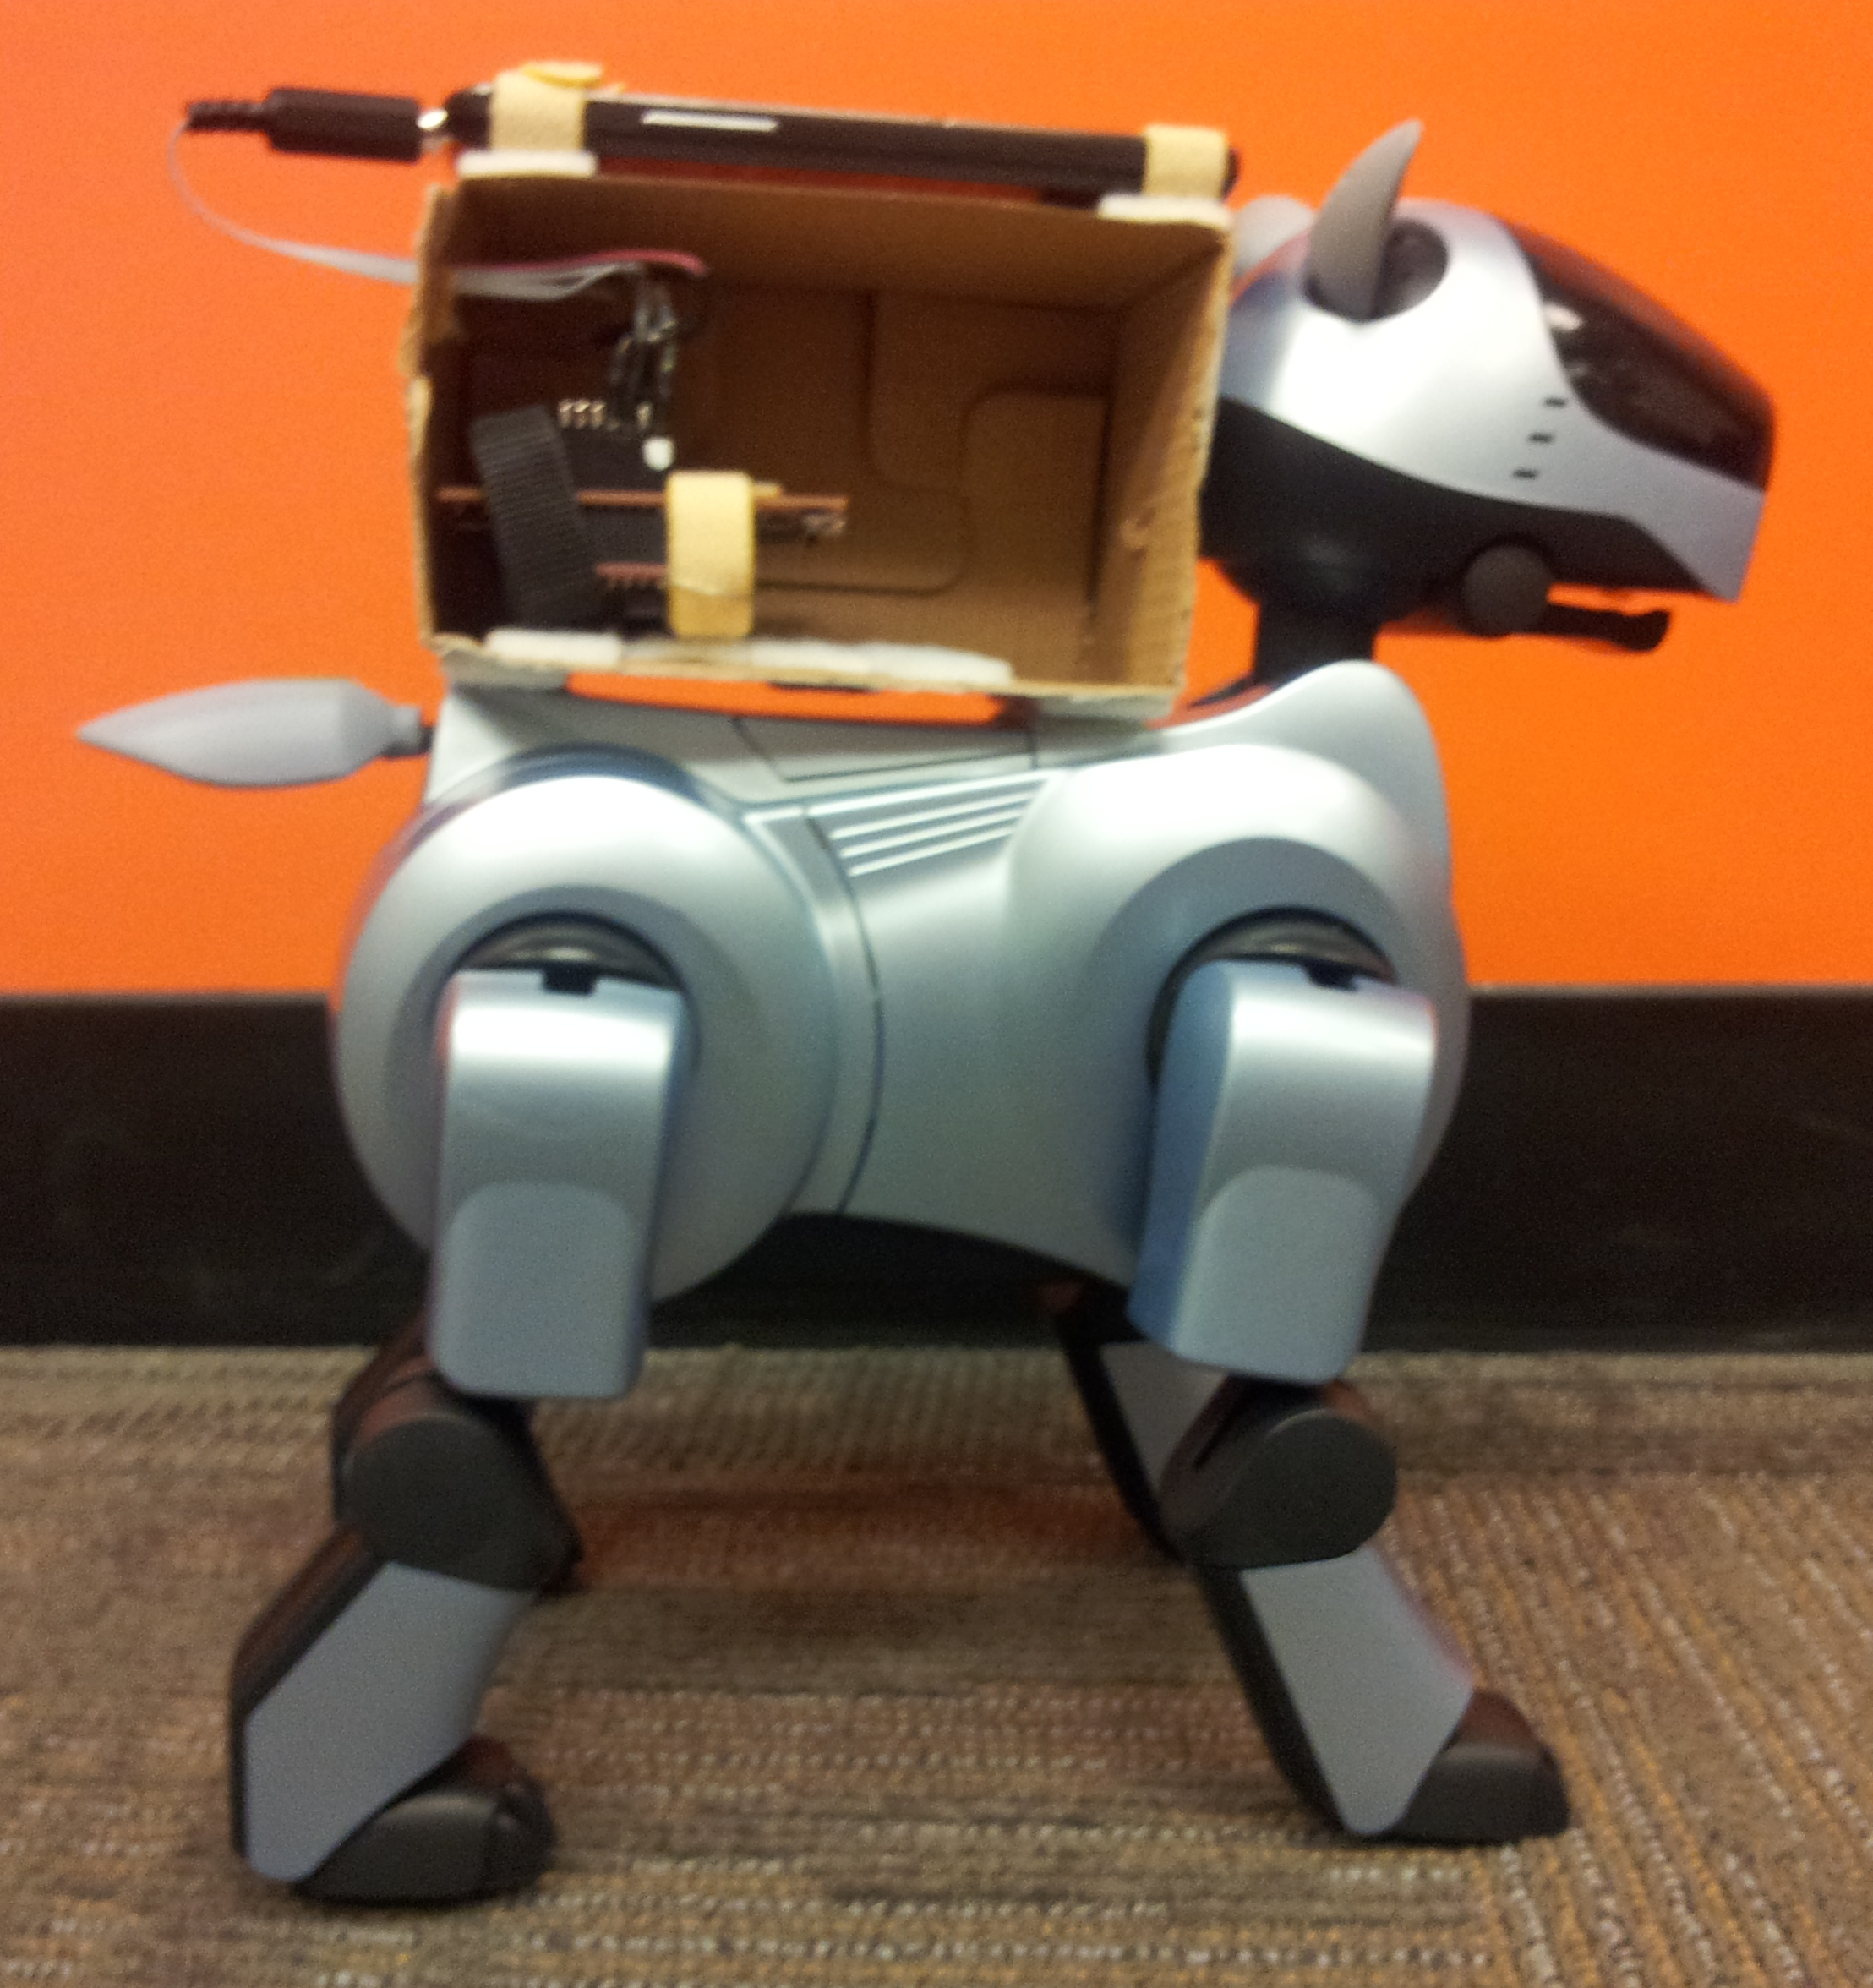
\includegraphics[width=3in]{aibo_ers_210.jpg}
	\caption{AIBO ERS 210 with Smartsensor prototype.}
	\label{fig:aibo}
\end{figure}

\subsection{Test Platform}
\label{sec:testPlatform}

To enable us to conduct controlled and repeatable experiments, we
mounted the prototype on the back of an AIBO ERA 210 robot
dog (see Figure~\ref{fig:aibo}).  Because the robot's actions can be
scripted, this setup provides an efficient and reliable way to
determine ground truth.  In contrast, labelling data collected from
human subjects with ground truth is error prone and labour intensive.

